
%  \documentclass{standalone}
%  \usepackage{currfile,hyperxmp}

% \input{../tikz_header.tex}
% \pgfplotsset{compat=newest}

%\begin{document}

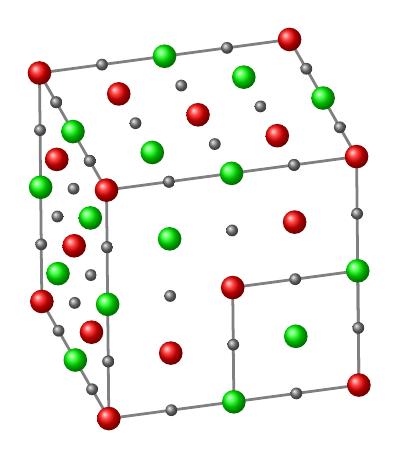
\begin{tikzpicture}[scale=2.5]
%\useasboundingbox (0,0) rectangle (5,5);
%\draw (2,2) rectangle ++(5,5);


 \begin{axis}[
   axis lines=none,
    xmin=-2.5,
    xmax=5.5,
    ymin=-2.5,
    ymax=5.5,
    zmin=-2.5,
    zmax=5.5,
    xtick=\empty,
    ytick=\empty,
    ztick=\empty,
    axis equal , rotate around z=40 ,rotate around x=-2 ,
    font=\footnotesize]

   
\newcommand{\Mnatom}{0.6mm}
\newcommand{\Oatom}{0.3mm}


\coordinate (0) at (0,0,0);
\coordinate (a) at (4,0,0);
\coordinate (b) at (0,4,0);
\coordinate (c) at (0,0,4);

\coordinate (abc) at (4,4,4);
\coordinate (ac) at (4,0,4);
\coordinate (bc) at (0,4,4);

\draw[gray] (0) -- (a) -- (ac) -- (c) -- (0) -- (b) -- (bc) -- (c);
\draw[gray] (bc) -- (abc) -- (ac) ;
\draw[gray] (4,0,0) -- (4,0,2) -- (2,0,2) -- (2,0,0);

\foreach \u in {0,1,2,3,4}{%  
\foreach \v in {0,1,2,3,4}{%  
    \edef\temp{%
    \noexpand\shade [ball color=gray](\u,\v,4) circle (\Oatom);
    \noexpand\shade [ball color=gray](\u,0,\v) circle (\Oatom);
    \noexpand\shade [ball color=gray](0,\u,\v) circle (\Oatom);
      }
   \temp
 } } 


\shade [ball color=red](0) circle (\Mnatom);

\shade [ball color=red](a) circle (\Mnatom);
\shade [ball color=red](b) circle (\Mnatom);
\shade [ball color=red](c) circle (\Mnatom);

\shade [ball color=red](abc) circle (\Mnatom);
\shade [ball color=red](ac) circle (\Mnatom);
\shade [ball color=red](bc) circle (\Mnatom);



\shade [ball color=red](1,0,1) circle (\Mnatom);
\shade [ball color=red](2,0,2) circle (\Mnatom);
\shade [ball color=red](3,0,3) circle (\Mnatom);

\shade [ball color=red](0,1,1) circle (\Mnatom);
\shade [ball color=red](0,2,2) circle (\Mnatom);
\shade [ball color=red](0,3,3) circle (\Mnatom);

\shade [ball color=red](3,1,4) circle (\Mnatom);
\shade [ball color=red](2,2,4) circle (\Mnatom);
\shade [ball color=red](1,3,4) circle (\Mnatom);


\shade [ball color=green](2,0,0) circle (\Mnatom);
\shade [ball color=green](3,0,1) circle (\Mnatom);
\shade [ball color=green](4,0,2) circle (\Mnatom);

\shade [ball color=green](0,0,2) circle (\Mnatom);
\shade [ball color=green](1,0,3) circle (\Mnatom);
\shade [ball color=green](2,0,4) circle (\Mnatom);

\shade [ball color=green](0,1,3) circle (\Mnatom);
\shade [ball color=green](0,2,4) circle (\Mnatom);

\shade [ball color=green](0,2,0) circle (\Mnatom);
\shade [ball color=green](0,3,1) circle (\Mnatom);
\shade [ball color=green](0,4,2) circle (\Mnatom);

\shade [ball color=green](1,1,4) circle (\Mnatom);

\shade [ball color=green](4,2,4) circle (\Mnatom);
\shade [ball color=green](3,3,4) circle (\Mnatom);
\shade [ball color=green](2,4,4) circle (\Mnatom);



  \end{axis}

  
  \end{tikzpicture}



%\end{document}